\section{Introduction}

\subsection{Motivation}
Assistive robots in domestic environments have the potential to aid persons with special needs in their daily living and can thereby help to maintain a quality of life that would otherwise be lost.
Robotic assistance can be beneficial to a variety of domains and users: The care and assistance of the elderly at home or in a nursing environment, assistance of persons with physical impairments and persons with cognitive or social deficits such as dementia or autism spectrum disorder.

It is estimated that the number of people above an age of 70 years in Germany will leap from 13 million to 19 million, i.e. increase by around $46\%$ over the next 20 years (see figure \ref{fig:population_germany}).
With the world's population growing older and caring facilities having reached their capacities already today, the need for assistive systems is specifically critical in elderly care.
Domestic robots may provide the freedom to keep living in the own home and prolong the time before living in an nursing environment becomes necessary.

\begin{figure}[H]
    \centering
    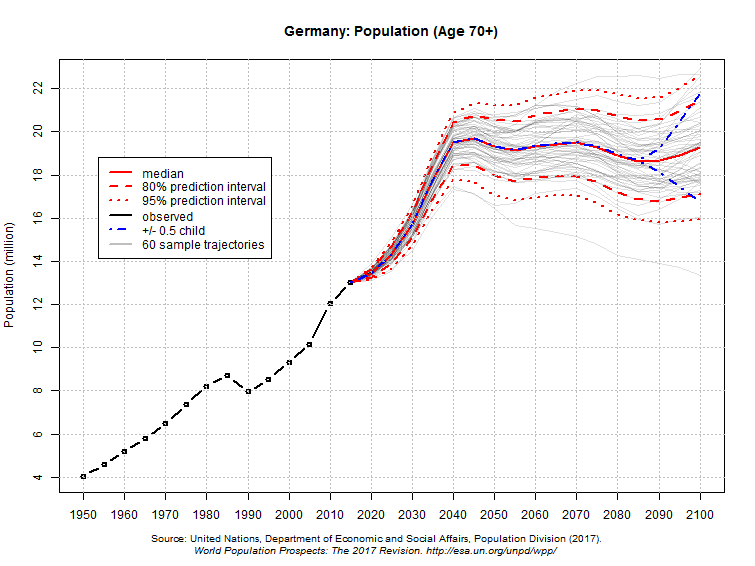
\includegraphics[width=\textwidth]{img_introduction/Germany.png}
    \caption{Estimation of the population of age 70+ in Germany}
    \label{fig:population_germany}
\end{figure}

Contact assistive robotics, i.e. robots with the ability to manipulate objects in their environment offer to perform simple every-day tasks for the physically impaired, the elderly and people in general need of help.
One of the biggest concerns in assistive robotics is to inadvertently harm someone \cite{mataric_socially_2016}.
Robots with manipulators, which represent additional powerful hardware, may raise the concern of possible harm and therefore resist widespread acceptance in e.g. elderly care.

In contrast, the field of socially assistive robotics aims at assisting persons through social rather than physical interaction \cite{feil-seifer_defining_2005}.
Examples include robotic animal toys, which aim at improving the physiological and psychological fitness of elderly persons through robotic interaction, like the robotic seal PARO \cite{wada_analysis_2002}.
Socially assistive robots have since been extended to a variety of helpful functions, such as intelligent reminding, cognitive stimulation and mobile videophony \cite{gross_progress_2011}.

This work is carried out in the context of the RoboLand project\footnote{\url{www.roboland-projekt.de}}, which aims at increasing social interactions for elderly persons with dementia in rural regions through telepresence.
Telepresence is an extended form of videophony through a remote controlled robot.
The market research institute \textit{Wainhouse Research} defines telepresence as ``a videoconferencing experience that creates the illusion that the remote participants are in the same room with you'' \cite{davis_telepresence_2007}.

Current telepresence robots span a wide spectrum of capabilities.
The initial two models that were selected for practical evaluation in the RoboLand project are:
\begin{description}
    \item[Double] \hfill\\
    A remote controlled self-balancing platform with an iPad attached to a telescopic retractable shaft.\footnote{\url{www.doublerobotics.com}} 
    \item[Amy] \hfill\\
    A ROS-based robotic platform, designed for telepresence and social assistance.
    In contrast to \textit{double}, \textit{Amy} is equipped with a variety of additional sensors, is able to perform autonomous robotics tasks such as navigation.
    These sensors include ultrasonic sensors, infrared sensors, an inertial measurement unit, a 2D camera and a 3D camera.\footnote{\url{www.amyrobotics.com}}
\end{description}


\subsection{Scope of this Work}
In order to provide assistance in a domestic environment, an autonomous assistive system first needs to know in what form and when assistance is required.
This can either be achieved by registering direct commands from the user, e.g. through voice recognition and touchscreen inputs or by autonomous recognition of visual stimuli from the system's environment.
By autonomously recognizing situations in which assistance is required, a robotic system is able to then offer a set of actions which could be executed to assist.
This provides a form of social immersion of the robot, since it is actively able to engage the user and offer assistance even if it might not actually be required. 

The underlying hypothesis of this work, is that currently performed actions by a human user are the best indicator for whether assistance is required or human-robot communication should be initiated.
This work therefore aims at providing a basis for improving assistive robotics through human action recognition from video data by an adapted deep learning approach, specifically for daily-living actions.

Since video cameras are a widespread and cheap technology, available in every mobile phone and naturally available in telepresence robots, a vast amount of video data is easily obtainable from video platforms such as YouTube for learning purposes.
An action recognition system that processes 2D video-data can therefore be easily deployed, since regular 2D cameras form the standard equipment of most robots.
In the context of the RoboLand project, we aim at extending the deployed robots beyond the telepresence functionality towards social assistance through human action recognition.

Action recognition is a classification task.
An action recognition system is presented with a video, usually a short clip that contains the performance of a single action, and then outputs the corresponding action class according to a finite and predefined set of recognizable actions.
In learning systems, this set of recognizable actions is defined by the labelling of the dataset that was used to train the system.

Deep learning approaches have shown remarkable results in a multitude of vision tasks.
These include tasks like hand-written digit recognition, object detection, scene labelling continue cite ??.
In our previously conducted literature survey, the performance of deep learning approaches in action recognition has been compared to the classical method of using hand-crafted features.
We concluded, that deep learning approaches do not yet outperform state-of-the-art hand-crafted feature methods, but show promising and competitive results.
We therefore aim to increase the performance of deep learning for action recognition further and specifically train a system for a recognizing daily-living actions, which could be deployed in the real-world on an assistive robotic system.

\subsection{Challenges}
The practical value of an action recognition system heavily depends on the data, that was used to train it, since it defines the action classes that can later be recognised.
Therefore a sufficiently large dataset of daily-living actions is necessary to obtain a classifier that can be used for recognising daily-living actions in a real-world setting.
The common disadvantage of deep neural networks, namely that they require a lot of labelled data in order to generalize effectively, has to be addressed.
Since manually collecting and labelling video-data is expensive, action recognition datasets are usually sampled from sources like movies, television broadcasts or online video platforms.
These videos however are often biased towards unrealistic or entertaining videos in staged and uncommon settings.
Traditionally, sports video have been used for general action recognition benchmarking datasets, since sports videos are widely distributed and a distinct label is easily obtainable.

Fortunately the work of \textcite{sigurdsson_hollywood_2016} already addressed the challenge of obtaining a dataset with \textit{boring} daily-living actions.
Since these types of actions are hard to sample from movies or the internet, a series of crowdsourced tasks was deployed to compile the dataset called Charades\textcite{sigurdsson_hollywood_2016}.
The complete process of creating actions scrips, recording the videos and annotating them with action labels was done by 267 individuals from three different continents.
The videos in the Charades dataset were recorded in regular homes by a decently large number of private actors.
It therefore contains a decent amount of variety in action performances in real-world scenes.
The dataset contains 9,848 videos with 66,500 individually labelled and temporally localized action instances.
The dataset was specifically to enable robotic applications in real-world environments.

The size of 66,500 action instances is extremely small for a deep learning dataset.
In comparison, the two currently biggest action recognition datasets are Sports-1M cite ?? (around one million noisily labelled sports videos) and YouTube-8M cite ?? (around eight million noisily labelled YouTube videos).
The practical benefit of these datasets however is questionable, since the labels are noisy and the contained actions are not temporally localized.
Recently, the Kinetics dataset was published, which addresses the issues of action recognition datasets being too small by providing ?? videos.
The actions in Kinetics are comparably well localized, since each video has a fixed length of 10 seconds which contains the action.
Even these datasets are magnitudes smaller compared to common image classification datasets.
EXAMPLES cite ??

In deep learning for action recognition two main approaches can be identified:
\begin{enumerate}
    \item
    Extending the convolutional kernels in regular (2D) CNNs to the temporal dimension and thereby enabling them to process 3D video volumes, that result from stacking consecutive video frames.
    One of the first publications that incorporate 3D CNNs for action recognition is \cite{ji_3d_2013}.
    \item
    Incorporation two separated processing streams of 2D CNNs into the overall network architecture. A spatial recognition stream processes RGB video frames and an additional temporal recognition stream receives optical flow inputs to incorporate explicit motion information. The prototypical publication that describes this approach is \cite{simonyan_two-stream_2014}.
\end{enumerate}

Our previously conducted survey cite ?? concludes that the two-stream approach in general performs better, than single-stream 3D convolutional networks.
The major deficiency of 3D convolutional neural networks is, that they treat the temporal and spatial domain equally.
A video volume of stacked input frames is treated as a regular 3D object.
However, the temporal dimension is not inherently equal to the spatial dimension, since adjacent frames correlate by obeying the laws of physics, i.e. shown objects cannot instantaneously disappear, move with finite velocities, so that the amount of change between frames is limited.

To address the above stated challenges, we incorporate an unsupervised pre-training strategy called \textit{temporal order verification}, which has previously shown to increase performance of 2D CNNs in action recognition.
During pre-training with \textit{temporal order verification} a model has to determine whether a presented input is in correct or incorrect order.
These inputs can be sampled from source videos by creating network inputs from the video frames and possibly permuting them.
This is in the strictest sense a supervised pre-training strategy.
However, since the labels \textit{correct temporal order} and \textit{incorrect temporal order} are automatically determined it is treated as an unsupervised method.
The obtained model weights are then used as initialization for training on the actual labelled dataset.

Pre-training a model with \textit{temporal order verification} has the following beneficial properties, which makes it particularly interesting for our work.
\begin{itemize}
    \item 
    since it basically is an unsupervised pre-training strategy, large amounts of possibly unlabelled video data can be incorporated in the pre-training process.
    \item
    \textcite{misra_shuffle_2016} describe the benefit of \textit{temporal order verification} in that the network needs to reason about the movement in the presented inputs, in order to determine the temporal order.
    The learned representations, therefore need to encode motion of the inputs, which is highly informative for the presented actions.
\end{itemize}

In this work, we investigate to transfer this pre-training strategy to a 3D CNN model, namely the \textit{C3D} convolutional network as described in \cite{tran_learning_2015}.
Our working hypothesis is, that \textit{temporal order verification} is especially beneficial for a single-stream 3D CNN in the domain of daily-living action recognition, because:
\begin{enumerate}
    \item
    There is not much labelled training data available that features \textit{boring} daily-living actions in real-world environments.
    Incorporating an unsupervised pre-training strategy addresses this problem.
    Specifically, the benefit of using the Kinetics dataset for pre-training is evaluated.
    \item 
    \textit{Temporal order verification} has shown to result in input representations that focus on human motion by comparing the temporal relations between inputs.
    Not treating the temporal dimension differently than the spatial dimension has previously been identified as the main deficit of 3D convolutional networks.
\end{enumerate}


\section{Related Work (Action Recognition)}

Field of action recognition can broadly be divided in classical hand-crafted feature based method and deep learning approaches.


\subsection{Overview}

\subsection{C3D}
The work of \textcite{tran_learning_2015} provides a prominent example of a 3D convolutional architecture, which does not require the explicit calculation of optical flow.
Optical flow has previously been incorporated in an additional temporal network stream by \textcite{simonyan_two-stream_2014}.
The network in \cite{tran_learning_2015} uses a volume of stacked video frames as input and therefore performs action recognition on raw RGB inputs only.
By training the network on the very large noisily labelled dataset Sports-1M \cite{karpathy_large-scale_2014}, the authors were able to train a generic spatio temporal feature extractor, which they call \textit{C3D}.
That is, the activations of the network's last fully connected layer can be used as a generic feature representation of the input.
An arbitrary classifier can then be trained on this input-representation to perform several differernt video-based vision tasks such as action recognition, scene classification or object detection.

The work of \textcite{karpathy_large-scale_2014} motivated the incorporation of 3D convolutions in \textit{C3D} by providing a comparative evaluation on different fusion strategies, i.e. on how to combine temporal and spatial information in different neural network architectures.
\textcite{tran_learning_2015} additionally conclude, the advantageous property of 3D convolutions, that temporal information is not immediately but gradualy condensed along the layer of a 3D CNN.

\begin{figure}[H]
    \centering
    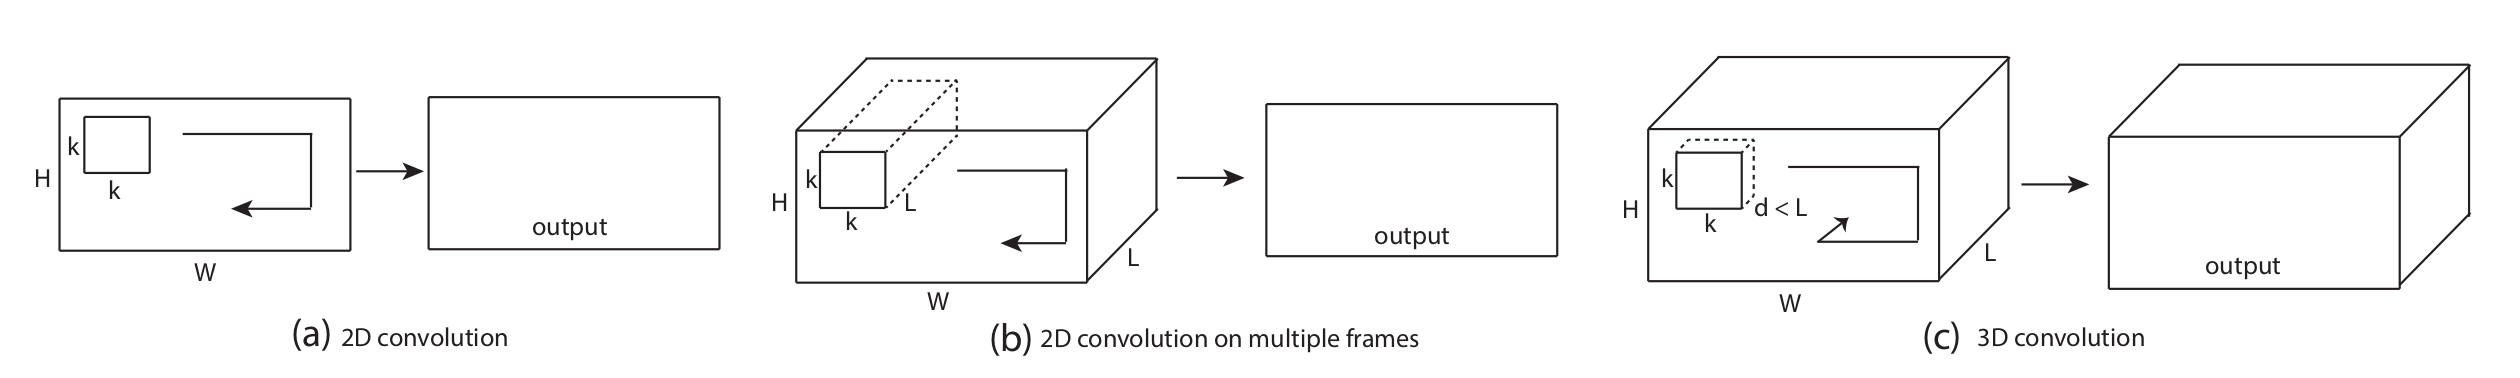
\includegraphics[width=\textwidth]{img_related/c3d_2dconv3dconv}
    \caption{Preservation of the temporal dimension by 3D convolutions: \textit{(a)} and \textit{(b)} 2D convolutions on a single or multiple frames results in a 2D feature map without temporal dimension. \textit{(c)} 3D convolutions on multiple input frames preserves the temporal dimension and results in a 3D feature map. \cite{tran_learning_2015}}
    \label{fig:c3d_2dconv3dconv}
\end{figure}

\textcite{tran_learning_2015} initially perform experiments on the smaller action recognition dataset UCF-101 \cite{soomro_ucf101:_2012}, to find the optimal size of kernels for the \textit{C3D} architecture. Results indicate, that kernels of size $3 \times 3 \times 3$ perform best.
The final architecture consists of 8 3D convolutional layers, 5 max-pooling layers, two fully-connected layers and a softmax output layer.
The architecture and layer sizes are illustrated in figure \ref{fig:c3d_architecture}.

\begin{figure}[H]
    \centering
    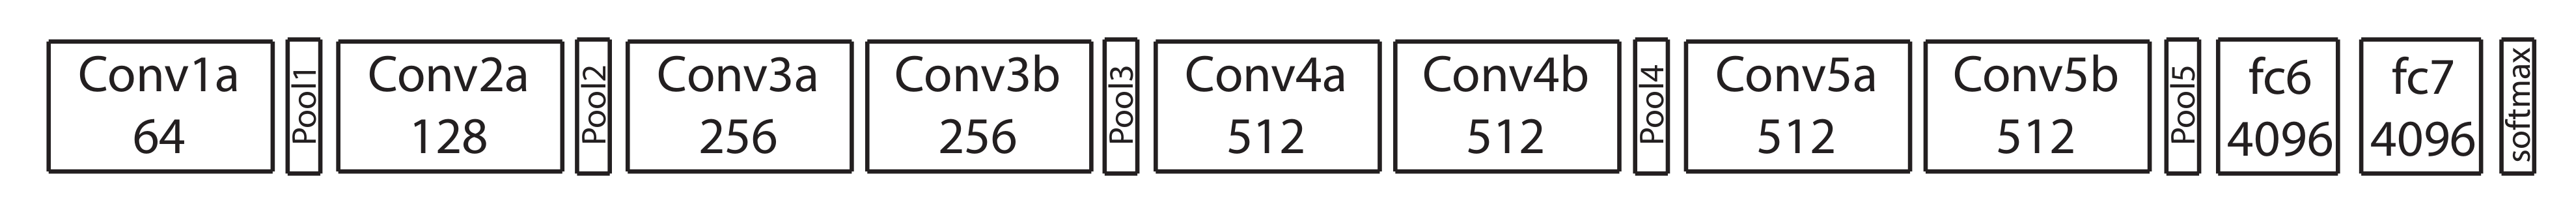
\includegraphics[width=\textwidth]{img_related/c3d_architecture}
    \caption{C3D architecture. Number of filters is given in each box. \cite{tran_learning_2015}}
    \label{fig:c3d_architecture}
\end{figure}

Final results when using a single \textit{C3D} network yield an accuracy of $82.3\%$ on UCF-101 \cite{soomro_ucf101:_2012}.
Note that these results were obtained from classifying the activations of the network's last fully-connected layer with an SVM.
The network was trained on the very large Sports-1M dataset \cite{karpathy_large-scale_2014} for this evaluation.
Only training the SVM on top of the networks activations uses the UCF-101 dataset.

Due to its competitive performance, the \textit{C3D} network is used as a prominent example of a 3D convolutional neural network using only raw RGB inputs.
\textcite{carreira_quo_2017} use it as main architecture to compare their own approach against.
Although the results of \textit{C3D} are competitive, the prototypical two-stream approach by \textcite{simonyan_two-stream_2014} outperforms \textit{C3D} by yielding $88.0\%$ accuracy on UCF-101.
Two-stream approaches are therefore considered the more successful architectures in action recognition \cite{wang_action_2015}, since they treat the spatial and temporal dimension differently.


\subsection{Temporal Order Verification}
\label{subsec:tov}

The work of \textcite{misra_shuffle_2016} is most related to ours.
The authors incorporate \textit{Temporal Coherency} between video frames to learn image representations, which are highly discriminative towards motion and therefore well suited for Action Recognition.
Our work is the logical continuation from learning these action representations with 2D CNNs as in \cite{misra_shuffle_2016} to 3D CNNs.

\textit{Temporal Coherency} describes an inherent relation between consecutive video frames.
More precisely, consecutive frames are semantically and dynamically correlated \cite{herath_going_2016}.
This means in terms of action recognition: Two consecutive frames are highly likely to present the same action and are limited by the laws of physics in the magnitute of change that can occur between them.

\textit{Temporal Coherency} can be used as a weak form of supervision in training deep networks, in contrast to strong supervision regular semantic labels.
\textcite{misra_shuffle_2016} propose an auxiliary quasi-unsupervised pre-training method which incorporates this \textit{Temporal Coherency} by first training a network on a binary classification task.
More precisely: The Network is presented with a sequence of input frames, which may have been randomly permuted, and has to determined if the sequence is in correct temporal order or not.
This pre-training task is called \textit{temporal order verification}.

This is, in the strictest sense, not an unsupervised training task, but since obtaining the label (\textit{correct temporal order} or \textit{incorrect temporal order}) is free, the authors attribute it as unsupervised \cite{misra_shuffle_2016}.
This has the advantage, that easily obtainable unlabelled data can be used for pre-training the network.

\textcite{misra_shuffle_2016} evaluate their approach by presenting three video frames to a triplet siamese CNN with 2D convolutions (see figure \ref{fig:shufflelearn_approach}).
Their results show, that using four or five frames did not result in an increase of performance.
Datasets utilized for training and evaluation are UCF-101 \cite{??} and HMDB-51 \cite{??}

\begin{figure}[H]
    \centering
    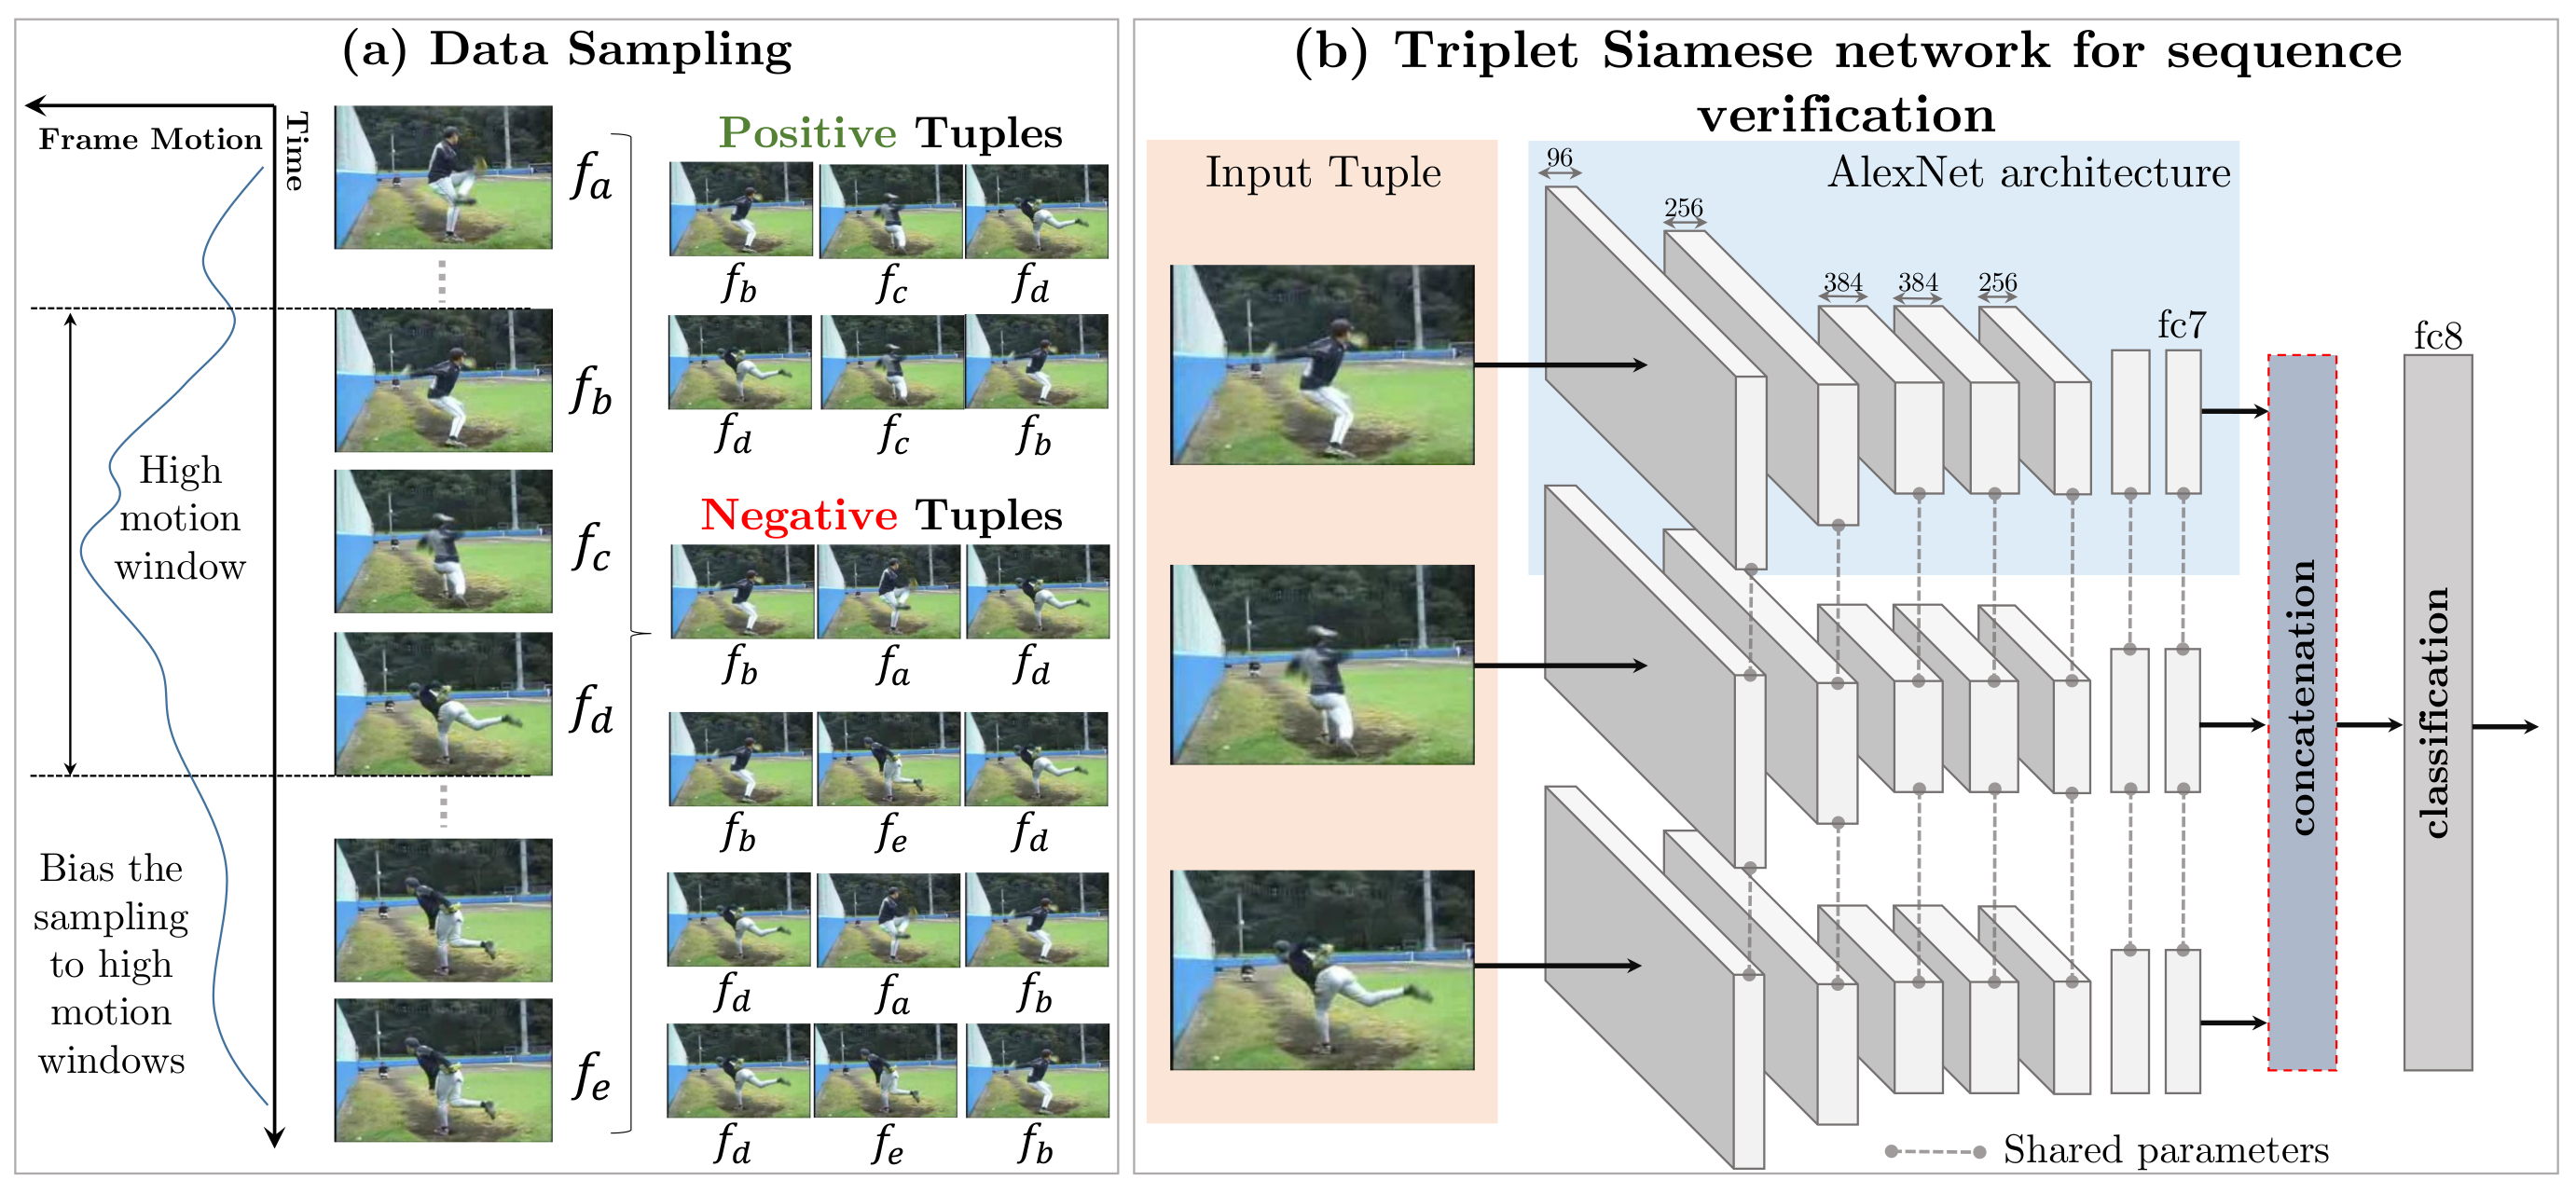
\includegraphics[width=\textwidth]{img_related/shufflelearn_approach}
    \caption{\textit{(Left)} Sampling of input sequences during temporal order verification. Sampling was biased towards regions with motion present in order to not obtain too similar frames. \textit{(Right)} Triplet siamese convolutional neural network, with shared weights. \cite{misra_shuffle_2016}}
    \label{fig:shufflelearn_approach}
\end{figure}

The authors use optical flow between two frames \cite{farneback_two-frame_2003} to identify a high motion window in the input video and construct positive examples (\textit{correct temporal order}) and negative examples (\textit{incorrect temporal order}) from the frames contained in it.
This ensures a certain magnitude of motion between the sampled frames and results in frame tuples, which are clearly distinguishable when permuted.

More precisely: Five frames $\{f_a, f_b, f_c, f_d, f_e\}$ are sampled from an input video, with $a < b < c < d < e$.
Out of these $f_a, f_b, f_c$ need to lie in the high motion window.
$f_b$ and $f_d$ are taken as start and end of the input sequence.
To construct a negative example (\textit{wrong temporal order}), $f_e$ or $f_a$ are inserted as middle frame to complete the input sequence.
The authors note, that it is vital to keep $f_b$ and $f_d$ as beginning and end of the input, i.e. the correct frames of the middle triple.
A mere inversion, i.e. $f_d, f_c, f_b$ is used as positive examples.

The incorporated network is available in the Caffe-Framework \cite{jia_caffe:_2014-1} and is called CaffeNet, an adapted version of the AlexNet model \cite{krizhevsky_imagenet_2012-1}.
The CNN model is arranged as a siamese triplet, with weight sharing.
That is: three identical copies of the network model each process one input frame, the results activations of the fully-connected layer are concatenated and then classified by an additional fully connected layer.
The individual network models share weights, i.e. each of them receive the same weight updates.

Results are obtained by training the composite model on UCF-101 and HMDB-51.
The model is either trained from scratch (weights are randomly initialized), pre-trained with \textit{temporal order verification} (weights are initialized from a pre-trained model) or pre-trained on UCF-101 for the evaluation on HMDB51.

\begin{table}[H]
    \centering
    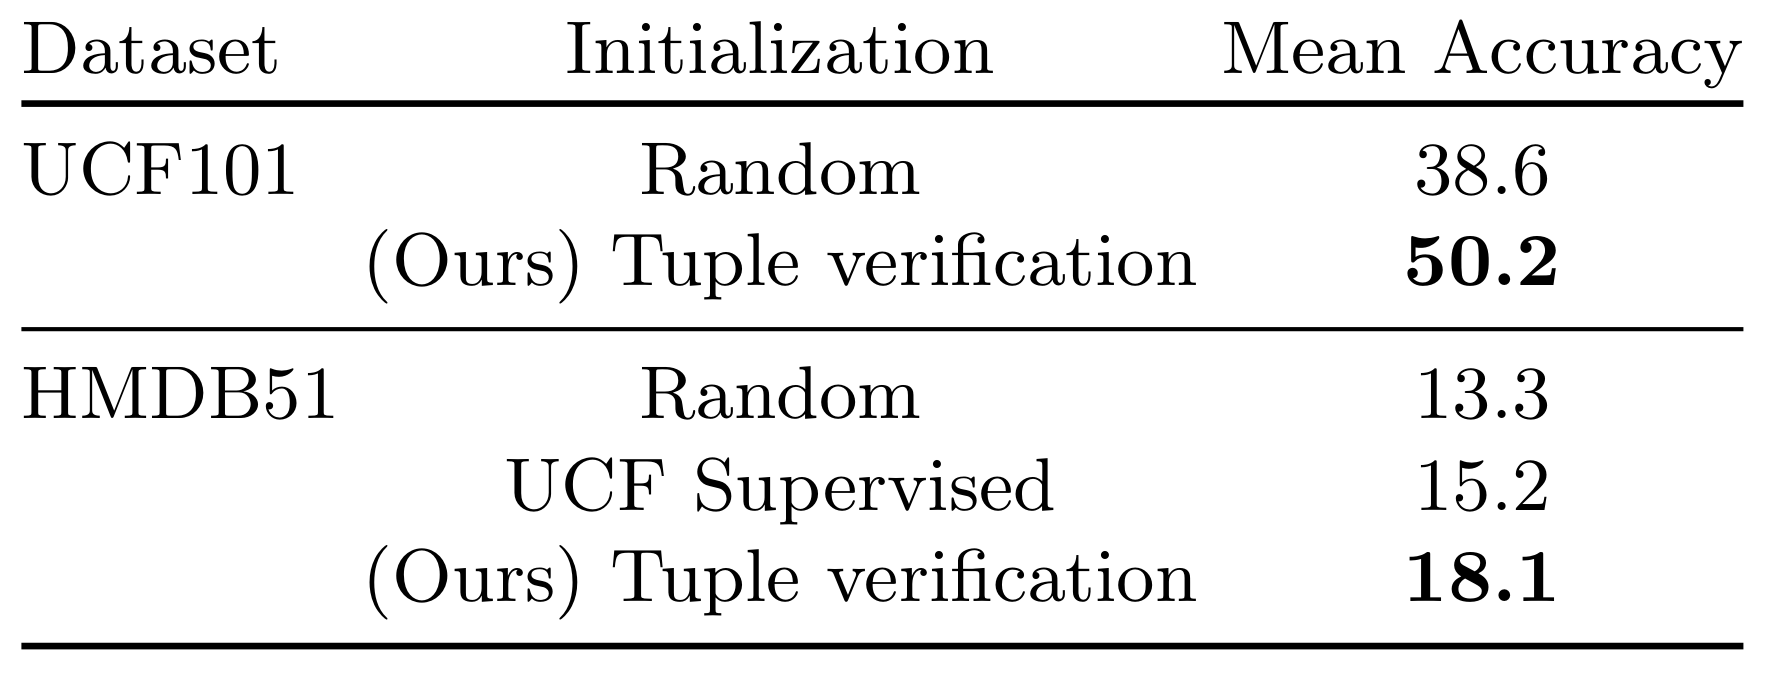
\includegraphics[width=0.6\textwidth]{img_related/shufflelearn_results}
    \caption{Perfomance gain in mean accuracy when incorporating temporal order verification as weight-initialization method on UCF-101 and HMDB-51 \cite{misra_shuffle_2016}}
    \label{tab:shufflelearn_results}
\end{table}

Table \ref{tab:shufflelearn_results} shows the increase in final performance after fine-tuning the model on either UCF-101 or HMDB-51.
The increase in performance of $+11.6\%$ is most prominent on UCF-101.
On HMDB-51 initializing the model using \textit{temporal order verification} achieves an increase in accuracy of $+4.8\%$, which is smaller than on UCF-101 but still significant.
Notably initialization from \textit{temporal order verification} outperforms initiliazing the network from regular pre-training on labeled data.
\bigskip

\textbf{Implementational details:}\\
\begin{itemize}
    \item The authors did not use any additional unlabeled data for pre-training, but sample around $900$k triples for \textit{temporal order verification} from the labeled datasets itself.
    \item Weights are randomly initialized for the \textit{temporal order verification} pre-training. 
    \item Pre-training is conducted for $100$k iterations with a fixed learning rate of $10^{-3}$ and a batch-size of 128 tuples (This results in around $14$ epochs in total for a pre-training set of $900$k triples).
    \item Best results were obtained with $25\%$ positive and $75\%$ negative triples.
    \item Batch normalization \cite{ioffe_batch_2017} is used during training.
    \item A single CaffeNet model is then initialized from the weights obtained from pre-training the siamese triplet. It is trained for $20$k iterations with a batch size of $256$ frames on UCF-101 and HMDB-51.
    \item The learning rate used for fine-tuning the model $10^{-2}$, which is decayed to $10^{-3}$ after $14$k iterations.
    \item Evaluation results are obtained from averaging random crops and flips from each test-video. First $25$ frames are uniformly sampled per video, $5$ input-sized regions are cropped out and flipped. This results in a total of $250$ inputs for averaging per video ($25$ frames $\times$ $5$ crops $\times$ $2$ flips).
\end{itemize}
